% Options for packages loaded elsewhere
\PassOptionsToPackage{unicode}{hyperref}
\PassOptionsToPackage{hyphens}{url}
%
\documentclass[
]{book}
\usepackage{amsmath,amssymb}
\usepackage{lmodern}
\usepackage{iftex}
\ifPDFTeX
  \usepackage[T1]{fontenc}
  \usepackage[utf8]{inputenc}
  \usepackage{textcomp} % provide euro and other symbols
\else % if luatex or xetex
  \usepackage{unicode-math}
  \defaultfontfeatures{Scale=MatchLowercase}
  \defaultfontfeatures[\rmfamily]{Ligatures=TeX,Scale=1}
\fi
% Use upquote if available, for straight quotes in verbatim environments
\IfFileExists{upquote.sty}{\usepackage{upquote}}{}
\IfFileExists{microtype.sty}{% use microtype if available
  \usepackage[]{microtype}
  \UseMicrotypeSet[protrusion]{basicmath} % disable protrusion for tt fonts
}{}
\makeatletter
\@ifundefined{KOMAClassName}{% if non-KOMA class
  \IfFileExists{parskip.sty}{%
    \usepackage{parskip}
  }{% else
    \setlength{\parindent}{0pt}
    \setlength{\parskip}{6pt plus 2pt minus 1pt}}
}{% if KOMA class
  \KOMAoptions{parskip=half}}
\makeatother
\usepackage{xcolor}
\IfFileExists{xurl.sty}{\usepackage{xurl}}{} % add URL line breaks if available
\IfFileExists{bookmark.sty}{\usepackage{bookmark}}{\usepackage{hyperref}}
\hypersetup{
  pdftitle={Exercise 5: Mapping with R},
  pdfauthor={Ben Davies},
  hidelinks,
  pdfcreator={LaTeX via pandoc}}
\urlstyle{same} % disable monospaced font for URLs
\usepackage{color}
\usepackage{fancyvrb}
\newcommand{\VerbBar}{|}
\newcommand{\VERB}{\Verb[commandchars=\\\{\}]}
\DefineVerbatimEnvironment{Highlighting}{Verbatim}{commandchars=\\\{\}}
% Add ',fontsize=\small' for more characters per line
\usepackage{framed}
\definecolor{shadecolor}{RGB}{248,248,248}
\newenvironment{Shaded}{\begin{snugshade}}{\end{snugshade}}
\newcommand{\AlertTok}[1]{\textcolor[rgb]{0.94,0.16,0.16}{#1}}
\newcommand{\AnnotationTok}[1]{\textcolor[rgb]{0.56,0.35,0.01}{\textbf{\textit{#1}}}}
\newcommand{\AttributeTok}[1]{\textcolor[rgb]{0.77,0.63,0.00}{#1}}
\newcommand{\BaseNTok}[1]{\textcolor[rgb]{0.00,0.00,0.81}{#1}}
\newcommand{\BuiltInTok}[1]{#1}
\newcommand{\CharTok}[1]{\textcolor[rgb]{0.31,0.60,0.02}{#1}}
\newcommand{\CommentTok}[1]{\textcolor[rgb]{0.56,0.35,0.01}{\textit{#1}}}
\newcommand{\CommentVarTok}[1]{\textcolor[rgb]{0.56,0.35,0.01}{\textbf{\textit{#1}}}}
\newcommand{\ConstantTok}[1]{\textcolor[rgb]{0.00,0.00,0.00}{#1}}
\newcommand{\ControlFlowTok}[1]{\textcolor[rgb]{0.13,0.29,0.53}{\textbf{#1}}}
\newcommand{\DataTypeTok}[1]{\textcolor[rgb]{0.13,0.29,0.53}{#1}}
\newcommand{\DecValTok}[1]{\textcolor[rgb]{0.00,0.00,0.81}{#1}}
\newcommand{\DocumentationTok}[1]{\textcolor[rgb]{0.56,0.35,0.01}{\textbf{\textit{#1}}}}
\newcommand{\ErrorTok}[1]{\textcolor[rgb]{0.64,0.00,0.00}{\textbf{#1}}}
\newcommand{\ExtensionTok}[1]{#1}
\newcommand{\FloatTok}[1]{\textcolor[rgb]{0.00,0.00,0.81}{#1}}
\newcommand{\FunctionTok}[1]{\textcolor[rgb]{0.00,0.00,0.00}{#1}}
\newcommand{\ImportTok}[1]{#1}
\newcommand{\InformationTok}[1]{\textcolor[rgb]{0.56,0.35,0.01}{\textbf{\textit{#1}}}}
\newcommand{\KeywordTok}[1]{\textcolor[rgb]{0.13,0.29,0.53}{\textbf{#1}}}
\newcommand{\NormalTok}[1]{#1}
\newcommand{\OperatorTok}[1]{\textcolor[rgb]{0.81,0.36,0.00}{\textbf{#1}}}
\newcommand{\OtherTok}[1]{\textcolor[rgb]{0.56,0.35,0.01}{#1}}
\newcommand{\PreprocessorTok}[1]{\textcolor[rgb]{0.56,0.35,0.01}{\textit{#1}}}
\newcommand{\RegionMarkerTok}[1]{#1}
\newcommand{\SpecialCharTok}[1]{\textcolor[rgb]{0.00,0.00,0.00}{#1}}
\newcommand{\SpecialStringTok}[1]{\textcolor[rgb]{0.31,0.60,0.02}{#1}}
\newcommand{\StringTok}[1]{\textcolor[rgb]{0.31,0.60,0.02}{#1}}
\newcommand{\VariableTok}[1]{\textcolor[rgb]{0.00,0.00,0.00}{#1}}
\newcommand{\VerbatimStringTok}[1]{\textcolor[rgb]{0.31,0.60,0.02}{#1}}
\newcommand{\WarningTok}[1]{\textcolor[rgb]{0.56,0.35,0.01}{\textbf{\textit{#1}}}}
\usepackage{longtable,booktabs,array}
\usepackage{calc} % for calculating minipage widths
% Correct order of tables after \paragraph or \subparagraph
\usepackage{etoolbox}
\makeatletter
\patchcmd\longtable{\par}{\if@noskipsec\mbox{}\fi\par}{}{}
\makeatother
% Allow footnotes in longtable head/foot
\IfFileExists{footnotehyper.sty}{\usepackage{footnotehyper}}{\usepackage{footnote}}
\makesavenoteenv{longtable}
\usepackage{graphicx}
\makeatletter
\def\maxwidth{\ifdim\Gin@nat@width>\linewidth\linewidth\else\Gin@nat@width\fi}
\def\maxheight{\ifdim\Gin@nat@height>\textheight\textheight\else\Gin@nat@height\fi}
\makeatother
% Scale images if necessary, so that they will not overflow the page
% margins by default, and it is still possible to overwrite the defaults
% using explicit options in \includegraphics[width, height, ...]{}
\setkeys{Gin}{width=\maxwidth,height=\maxheight,keepaspectratio}
% Set default figure placement to htbp
\makeatletter
\def\fps@figure{htbp}
\makeatother
\setlength{\emergencystretch}{3em} % prevent overfull lines
\providecommand{\tightlist}{%
  \setlength{\itemsep}{0pt}\setlength{\parskip}{0pt}}
\setcounter{secnumdepth}{5}
\usepackage{booktabs}
\ifLuaTeX
  \usepackage{selnolig}  % disable illegal ligatures
\fi
\usepackage[]{natbib}
\bibliographystyle{plainnat}

\title{Exercise 5: Mapping with R}
\author{Ben Davies}
\date{2022-05-11}

\begin{document}
\maketitle

{
\setcounter{tocdepth}{1}
\tableofcontents
}
\hypertarget{making-maps-with-r}{%
\chapter{Making maps with R}\label{making-maps-with-r}}

With the help of many user generated packages, R can operate as a full-fledged geographic information system. One place where R truly shines over many desktop GIS platforms is the control a user has over the display of spatial information. While R's base graphics capabilities are useful for quickly visualizing data, packages like \texttt{ggplot2} and others offer cleaner default plotting and specialize in manipulating all aspects of a plot's appearance. Here, we will explore some of these capabilities for mapped data.

\hypertarget{adding-packages}{%
\section{Adding packages}\label{adding-packages}}

While \texttt{sf} and \texttt{terra} are useful for handling spatial data, they aren't built for visualization. To help us out, we're going to add some packages from the \texttt{ggplot2} family:

\begin{Shaded}
\begin{Highlighting}[]
\FunctionTok{require}\NormalTok{(}\StringTok{"sf"}\NormalTok{)}
\end{Highlighting}
\end{Shaded}

\begin{verbatim}
## Loading required package: sf
\end{verbatim}

\begin{verbatim}
## Linking to GEOS 3.9.1, GDAL 3.3.2, PROJ 7.2.1; sf_use_s2() is TRUE
\end{verbatim}

\begin{Shaded}
\begin{Highlighting}[]
\FunctionTok{require}\NormalTok{(}\StringTok{"terra"}\NormalTok{)}
\end{Highlighting}
\end{Shaded}

\begin{verbatim}
## Loading required package: terra
\end{verbatim}

\begin{verbatim}
## terra 1.5.21
\end{verbatim}

\begin{Shaded}
\begin{Highlighting}[]
\FunctionTok{require}\NormalTok{(}\StringTok{"ggplot2"}\NormalTok{) }\CommentTok{\# main graphics package}
\end{Highlighting}
\end{Shaded}

\begin{verbatim}
## Loading required package: ggplot2
\end{verbatim}

\begin{verbatim}
## 
## Attaching package: 'ggplot2'
\end{verbatim}

\begin{verbatim}
## The following object is masked from 'package:terra':
## 
##     arrow
\end{verbatim}

\begin{Shaded}
\begin{Highlighting}[]
\FunctionTok{require}\NormalTok{(}\StringTok{"ggspatial"}\NormalTok{) }\CommentTok{\# map specific ggplot functionality}
\end{Highlighting}
\end{Shaded}

\begin{verbatim}
## Loading required package: ggspatial
\end{verbatim}

Just a little background: the \texttt{ggplot2} package was developed in 2005 by \href{https://hadley.nz/}{Hadley Wickham} as a software approach to visualization scheme called \href{https://link.springer.com/book/10.1007/0-387-28695-0}{``The Grammar of Graphics''} published by Leland Wilkinson. The major distinction between \texttt{base} graphics and \texttt{ggplot2} is the ability to control the elements of a plot as a series of layers that can be added, shuffled, or removed.

\hypertarget{getting-going-with-ggplot2-and-geom_sf}{%
\chapter{\texorpdfstring{Getting going with \texttt{ggplot2} and \texttt{geom\_sf}}{Getting going with ggplot2 and geom\_sf}}\label{getting-going-with-ggplot2-and-geom_sf}}

Over the years, the developers of \texttt{ggplot2} have recognized widespread interest in using the package to make maps, and have updated the software to include handling and plotting of spatial data At the same time, efforts like the promotion of the Simple Features data structure are a recognition that data interoperability is a priority for many data users.

These two processes meet in the middle with the \texttt{geom\_sf} object. This is a way of translating Simple Features data (like that from the \texttt{sf} package) into a format that can be manipulated in the \texttt{ggplot2} environment. The general scheme looks something like this:

\begin{Shaded}
\begin{Highlighting}[]
\CommentTok{\#Plot a blank geom\_sf object}
\FunctionTok{ggplot}\NormalTok{() }\SpecialCharTok{+} \FunctionTok{geom\_sf}\NormalTok{()}
\end{Highlighting}
\end{Shaded}

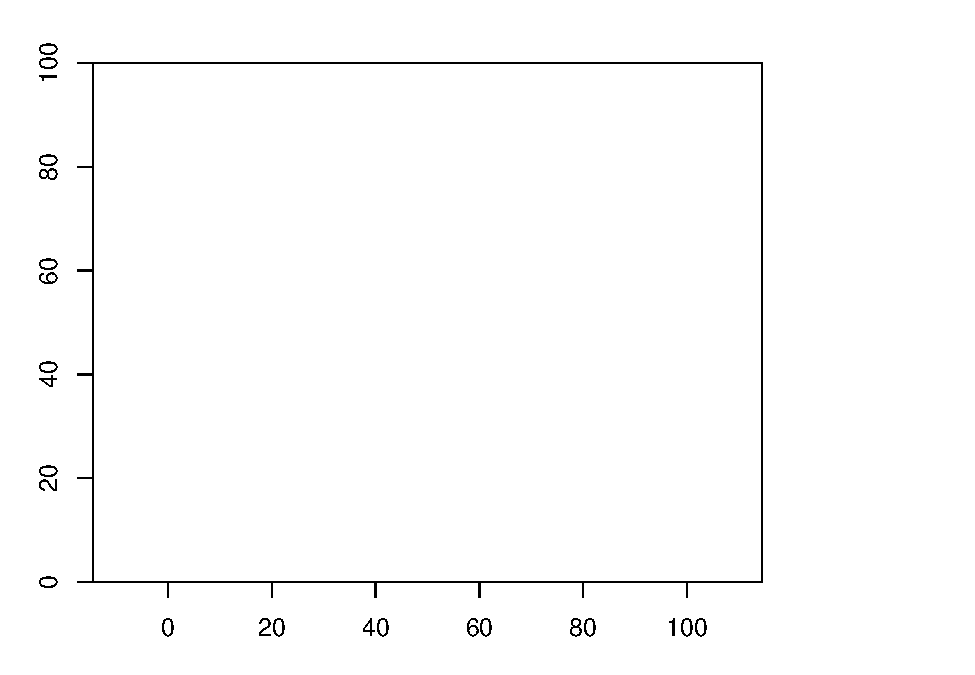
\includegraphics{_main_files/figure-latex/unnamed-chunk-3-1.pdf}
This begins with an empty \texttt{ggplot} object. To this we add (with the \texttt{+} operator) a \texttt{geom\_sf} object. In order to plot data, though, this will need some data.

\hypertarget{add-some-data}{%
\section{Add some data}\label{add-some-data}}

The dataset we'll start with are white-bearded wildebeest tracks at three study areas in Kenya, downloaded from \href{https://www.movebank.org/cms/webapp?gwt_fragment=page=studies,path=study208413731}{Movebank}.

\begin{Shaded}
\begin{Highlighting}[]
\CommentTok{\#Load data}
\NormalTok{wbTracks}\OtherTok{\textless{}{-}}\FunctionTok{st\_read}\NormalTok{(}\StringTok{"wildebeestTracks.shp"}\NormalTok{)}
\end{Highlighting}
\end{Shaded}

\begin{verbatim}
## Reading layer `wildebeestTracks' from data source 
##   `C:\Users\bdav_\Dropbox\Teaching\Spatial R Short Course\Bookdown\Exercise5\Exercise5\wildebeestTracks.shp' 
##   using driver `ESRI Shapefile'
## replacing null geometries with empty geometries
## Simple feature collection with 46 features and 1 field (with 10 geometries empty)
## Geometry type: LINESTRING
## Dimension:     XY
## Bounding box:  xmin: 34.80902 ymin: -2.957671 xmax: 37.71177 ymax: -1.114714
## Geodetic CRS:  WGS 84
\end{verbatim}

This is linestring data, so we should be expecting lines in our plot.

\hypertarget{plotting-a-geom_sf-object}{%
\section{\texorpdfstring{Plotting a \texttt{geom\_sf} object}{Plotting a geom\_sf object}}\label{plotting-a-geom_sf-object}}

We can add it to our blank object this way:

\begin{Shaded}
\begin{Highlighting}[]
\CommentTok{\#Plot sf linestring data}
\FunctionTok{ggplot}\NormalTok{() }\SpecialCharTok{+} 
  \FunctionTok{geom\_sf}\NormalTok{(}\AttributeTok{data =}\NormalTok{ wbTracks)}
\end{Highlighting}
\end{Shaded}

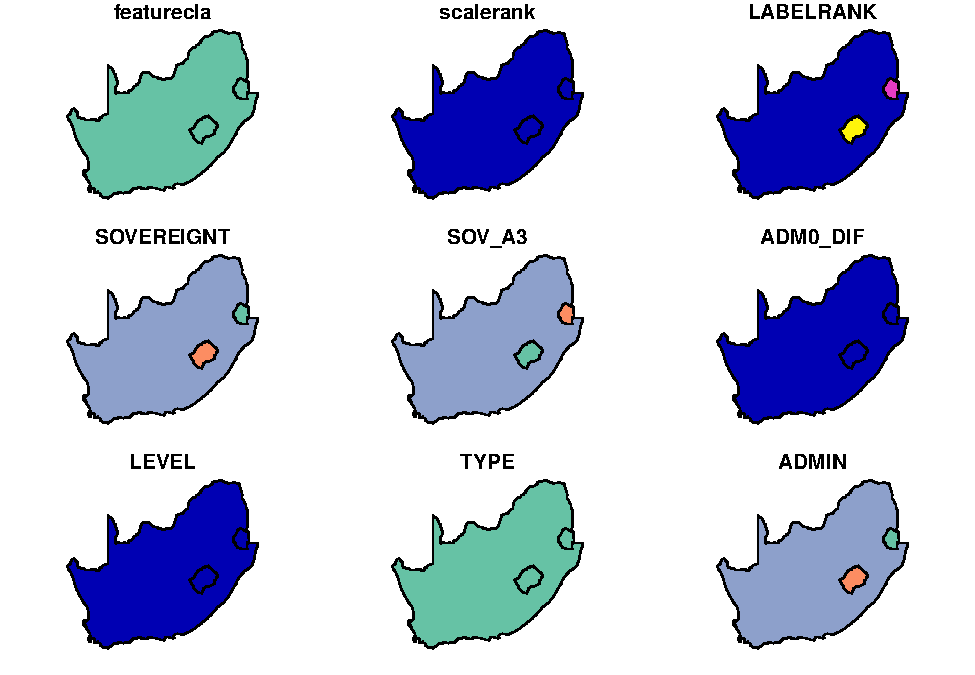
\includegraphics{_main_files/figure-latex/unnamed-chunk-5-1.pdf}

Looks like tracks to me! Note that we need to put \texttt{data=} before the dataset in our \texttt{geom\_sf} call. This tells ggplot2 that what we're passing it is not meant to be something other than data (it's not so good at guessing).

\hypertarget{changing-appearances}{%
\section{Changing appearances}\label{changing-appearances}}

First, let's have a look at this data.

\begin{Shaded}
\begin{Highlighting}[]
\CommentTok{\#Look at first six lines of data}
\FunctionTok{head}\NormalTok{(wbTracks)}
\end{Highlighting}
\end{Shaded}

\begin{verbatim}
## Simple feature collection with 6 features and 1 field
## Geometry type: LINESTRING
## Dimension:     XY
## Bounding box:  xmin: 34.83135 ymin: -2.957671 xmax: 35.75016 ymax: -1.114714
## Geodetic CRS:  WGS 84
##            name                       geometry
## 1 Naboisho-2829 LINESTRING (35.30873 -1.343...
## 2    Naiba-2830 LINESTRING (35.37816 -1.381...
## 3  Kayioni-2831 LINESTRING (35.31887 -1.333...
## 4    Nagol-2832 LINESTRING (35.4046 -1.3339...
## 5  Koyiaki-2833 LINESTRING (35.32003 -1.390...
## 6  Naisula-2834 LINESTRING (35.67744 -1.299...
\end{verbatim}

The name of the animal is the only piece of information here, so we'll use that to change the look of the plot.

\begin{Shaded}
\begin{Highlighting}[]
\CommentTok{\#Plot with lines colored by animal}
\FunctionTok{ggplot}\NormalTok{() }\SpecialCharTok{+} 
  \FunctionTok{geom\_sf}\NormalTok{(}\AttributeTok{data =}\NormalTok{ wbTracks, }\FunctionTok{aes}\NormalTok{(}\AttributeTok{color=}\NormalTok{name))}
\end{Highlighting}
\end{Shaded}

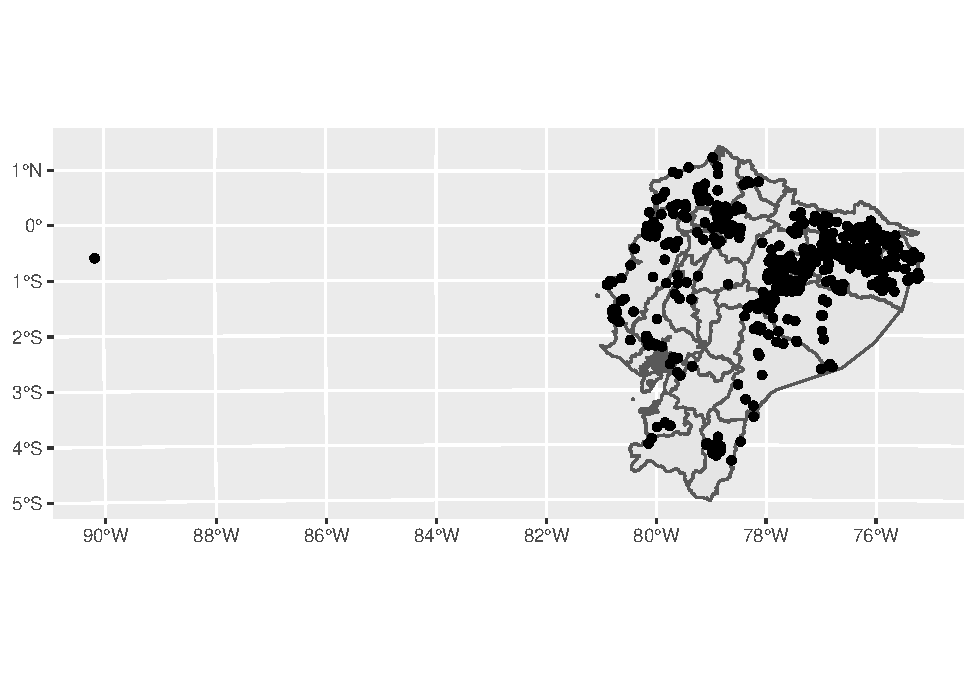
\includegraphics{_main_files/figure-latex/unnamed-chunk-7-1.pdf}

Eek! The legend takes up almost the whole image! Let's get rid of that for now. To do this, we add another element with \texttt{+}, and then use \texttt{theme()} to modify the legend settings:

\begin{Shaded}
\begin{Highlighting}[]
\CommentTok{\#Plot without legend}
\FunctionTok{ggplot}\NormalTok{() }\SpecialCharTok{+} 
  \FunctionTok{geom\_sf}\NormalTok{(}\AttributeTok{data =}\NormalTok{ wbTracks, }\FunctionTok{aes}\NormalTok{(}\AttributeTok{color=}\NormalTok{name)) }\SpecialCharTok{+}
  \FunctionTok{theme}\NormalTok{(}\AttributeTok{legend.position=}\DecValTok{0}\NormalTok{)}
\end{Highlighting}
\end{Shaded}

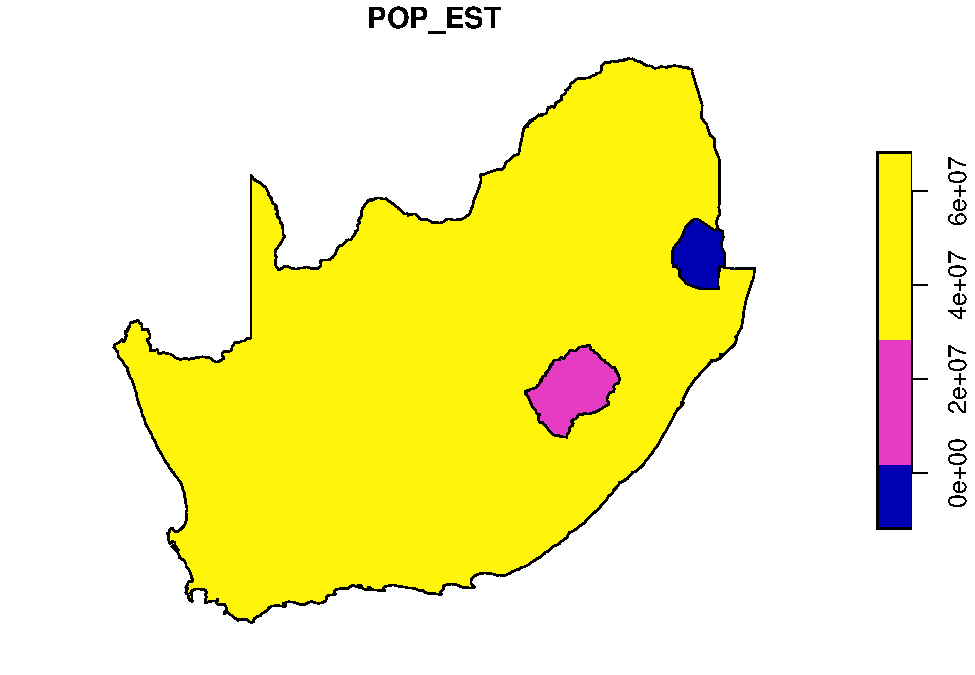
\includegraphics{_main_files/figure-latex/unnamed-chunk-8-1.pdf}

That's better. Each ggplot object has a \emph{theme} that controls aspects of the plot that are unrelated to the data. What we did there was pass an argument about the position, which could be a set of coordinates The default is \texttt{theme\_grey}, but there are a number of \href{https://ggplot2.tidyverse.org/reference/ggtheme.html}{preset themes} that we can use. For example\ldots{}

\begin{Shaded}
\begin{Highlighting}[]
\CommentTok{\#Plot with theme\_bw() theme}
\FunctionTok{ggplot}\NormalTok{() }\SpecialCharTok{+} 
  \FunctionTok{geom\_sf}\NormalTok{(}\AttributeTok{data =}\NormalTok{ wbTracks, }\FunctionTok{aes}\NormalTok{(}\AttributeTok{color=}\NormalTok{name)) }\SpecialCharTok{+}
  \FunctionTok{theme\_bw}\NormalTok{() }\SpecialCharTok{+}
  \FunctionTok{theme}\NormalTok{(}\AttributeTok{legend.position=}\DecValTok{0}\NormalTok{)}
\end{Highlighting}
\end{Shaded}

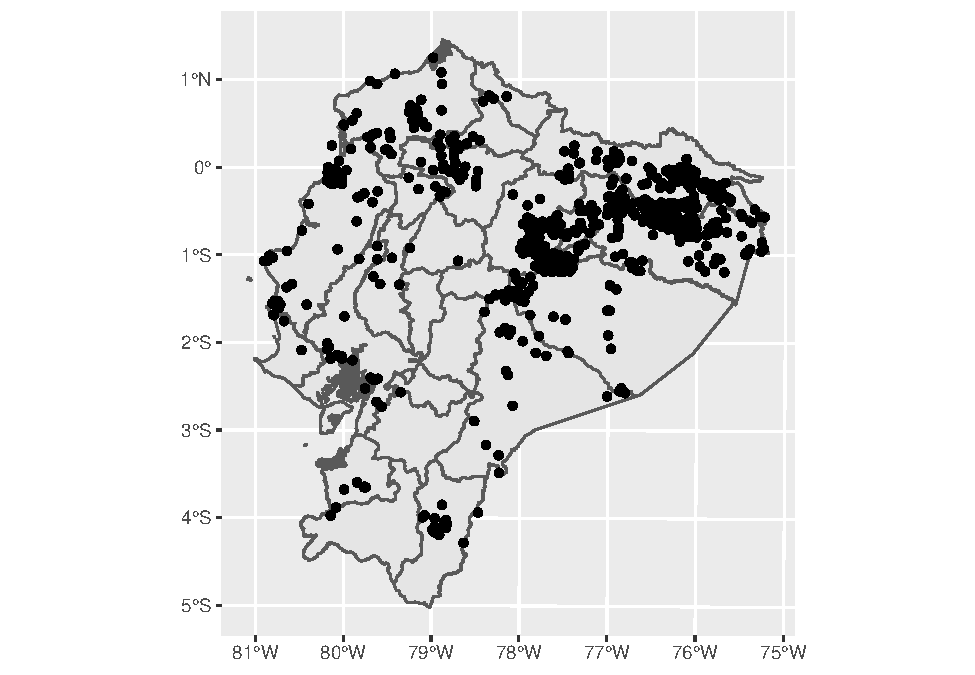
\includegraphics{_main_files/figure-latex/unnamed-chunk-9-1.pdf}

\ldots or this\ldots{}

\begin{Shaded}
\begin{Highlighting}[]
\CommentTok{\#Plot with theme\_dark() theme}
\FunctionTok{ggplot}\NormalTok{() }\SpecialCharTok{+} 
  \FunctionTok{geom\_sf}\NormalTok{(}\AttributeTok{data =}\NormalTok{ wbTracks, }\FunctionTok{aes}\NormalTok{(}\AttributeTok{color=}\NormalTok{name)) }\SpecialCharTok{+}
  \FunctionTok{theme\_dark}\NormalTok{() }\SpecialCharTok{+}
  \FunctionTok{theme}\NormalTok{(}\AttributeTok{legend.position=}\DecValTok{0}\NormalTok{)}
\end{Highlighting}
\end{Shaded}

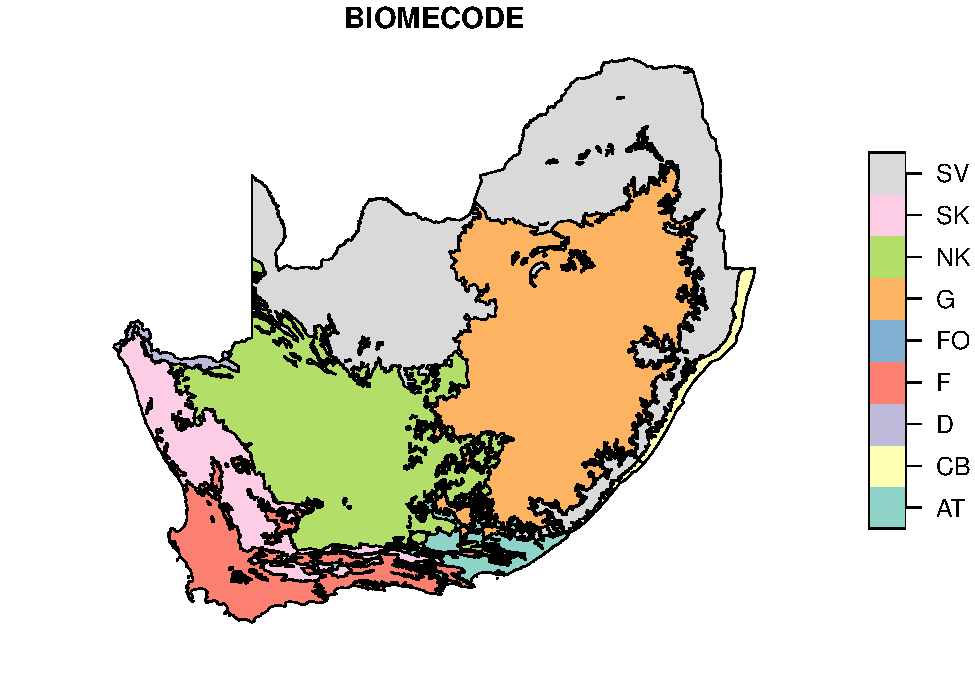
\includegraphics{_main_files/figure-latex/unnamed-chunk-10-1.pdf}

For now we'll stick with the grey theme. There are other elements we might add to this plot. For example, there are no axis labels or title here. There are specific calls we can make for these elements:

\begin{Shaded}
\begin{Highlighting}[]
\CommentTok{\#Plot with title and axis labels}
\FunctionTok{ggplot}\NormalTok{() }\SpecialCharTok{+} 
  \FunctionTok{geom\_sf}\NormalTok{(}\AttributeTok{data =}\NormalTok{ wbTracks, }\FunctionTok{aes}\NormalTok{(}\AttributeTok{color=}\NormalTok{name)) }\SpecialCharTok{+}
  \FunctionTok{theme\_grey}\NormalTok{() }\SpecialCharTok{+}
  \FunctionTok{theme}\NormalTok{(}\AttributeTok{legend.position=}\DecValTok{0}\NormalTok{) }\SpecialCharTok{+}
  \FunctionTok{xlab}\NormalTok{(}\StringTok{"Longitude"}\NormalTok{) }\SpecialCharTok{+}
  \FunctionTok{ylab}\NormalTok{(}\StringTok{"Latitude"}\NormalTok{) }\SpecialCharTok{+}
  \FunctionTok{ggtitle}\NormalTok{(}\StringTok{"White{-}Bearded Wildebeest"}\NormalTok{)}
\end{Highlighting}
\end{Shaded}

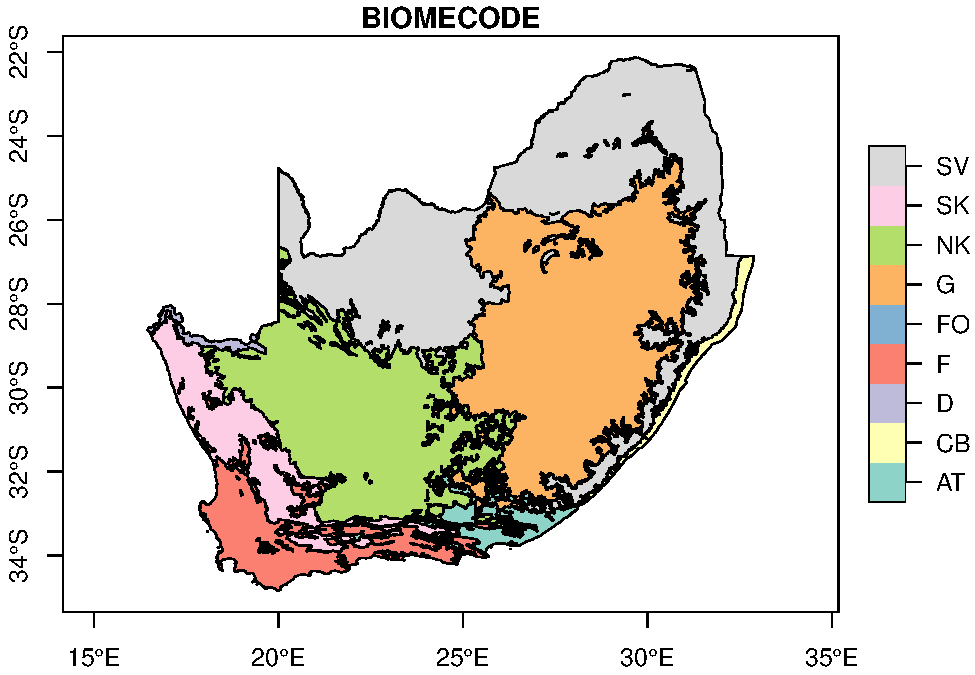
\includegraphics{_main_files/figure-latex/unnamed-chunk-11-1.pdf}

Alternatively, these can be done with the \texttt{labs()} object:

\begin{Shaded}
\begin{Highlighting}[]
\CommentTok{\#Plot with title and axis labels}
\FunctionTok{ggplot}\NormalTok{() }\SpecialCharTok{+} 
  \FunctionTok{geom\_sf}\NormalTok{(}\AttributeTok{data =}\NormalTok{ wbTracks, }\FunctionTok{aes}\NormalTok{(}\AttributeTok{color=}\NormalTok{name)) }\SpecialCharTok{+}
  \FunctionTok{theme\_grey}\NormalTok{() }\SpecialCharTok{+}
  \FunctionTok{theme}\NormalTok{(}\AttributeTok{legend.position=}\DecValTok{0}\NormalTok{) }\SpecialCharTok{+}
  \FunctionTok{labs}\NormalTok{(}\AttributeTok{x=}\StringTok{"Longitude"}\NormalTok{,}\AttributeTok{y=}\StringTok{"Latitude"}\NormalTok{,}\AttributeTok{title=}\StringTok{"White{-}Bearded Wildebeest"}\NormalTok{)}
\end{Highlighting}
\end{Shaded}

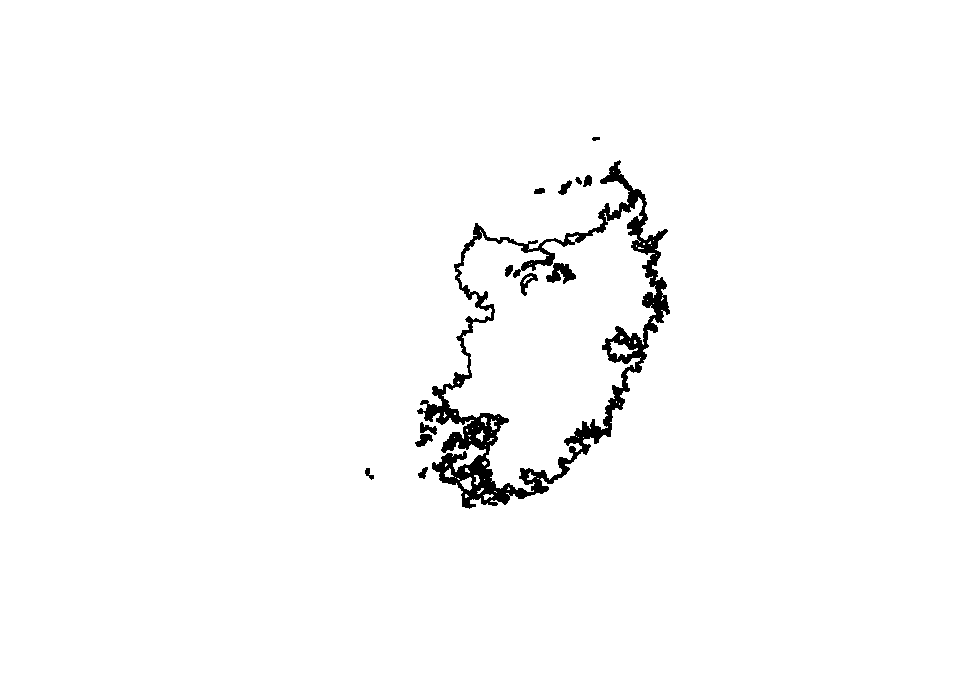
\includegraphics{_main_files/figure-latex/unnamed-chunk-12-1.pdf}

This is just a brief introduction to plotting controls with \texttt{ggplot2}. You could take an entire course on data visualization with this package and still only scratch the surface. For more about this, the book \href{https://ggplot2-book.org/}{ggplot2: Elegant Graphics for Data Analysis} is free and offers a very thorough treatment.

\hypertarget{try-it-yourself}{%
\section{Try it yourself!}\label{try-it-yourself}}

In this section we plotted the tracks using the default color scheme, but there's a lot of different options for this.
* Try adding another element to this plot using the \texttt{scale\_fill\_brewer()} function. This can take a \texttt{palette=} argument, which you can plug in the name of a ColorBrewer palette. Try a few! The names can be found \href{http://applied-r.com/rcolorbrewer-palettes/}{here}.

\hypertarget{mapping-multiple-datasets}{%
\chapter{Mapping multiple datasets}\label{mapping-multiple-datasets}}

OK, now we have seen how to make maps with a single dataset. There's some things to keep in mind when working with multiple datasets. This section will look at this process.

\hypertarget{add-data}{%
\section{Add data}\label{add-data}}

This first dataset is primate species observation data from the \href{https://www.gbif.org/}{Global Biodiversity Information Facility (GBIF)}, covering all of South America. It is in CSV format, so we need to use \texttt{st\_as\_sf} to convert it to an \texttt{sf} object:

\begin{Shaded}
\begin{Highlighting}[]
\CommentTok{\#Load data}
\NormalTok{primateObs}\OtherTok{\textless{}{-}}\FunctionTok{read.csv}\NormalTok{(}\StringTok{"SAPrimateObservations.csv"}\NormalTok{)}
\NormalTok{primates}\OtherTok{\textless{}{-}}\FunctionTok{st\_as\_sf}\NormalTok{(primateObs,}\AttributeTok{coords=}\FunctionTok{c}\NormalTok{(}\StringTok{"decimalLongitude"}\NormalTok{,}\StringTok{"decimalLatitude"}\NormalTok{))}
\FunctionTok{st\_crs}\NormalTok{(primates)}\OtherTok{\textless{}{-}}\StringTok{"EPSG:4326"}
\FunctionTok{plot}\NormalTok{(}\FunctionTok{st\_geometry}\NormalTok{(primates))}
\end{Highlighting}
\end{Shaded}

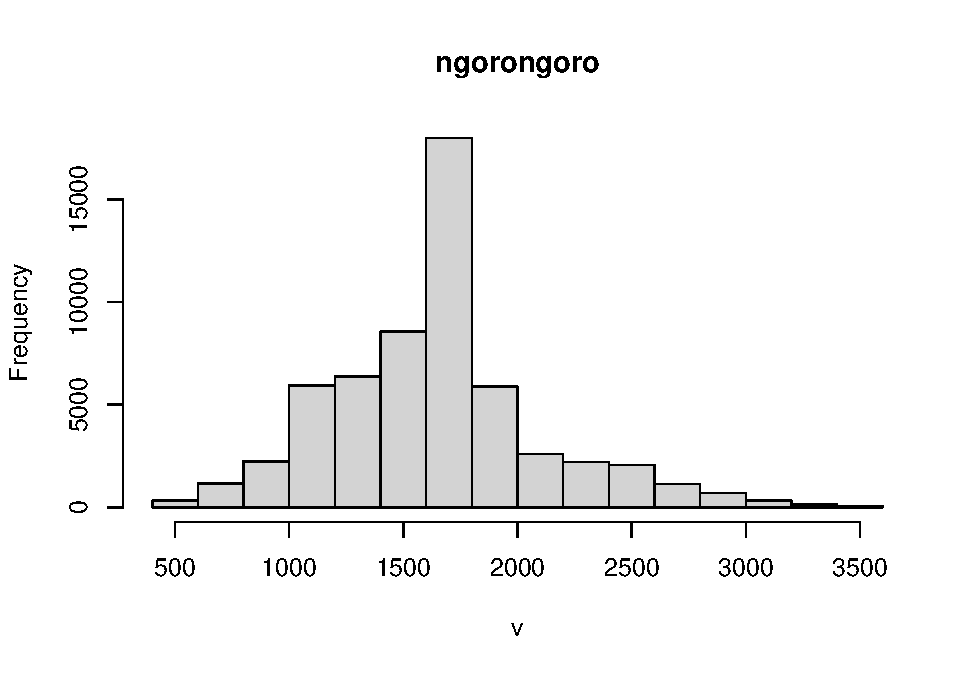
\includegraphics{_main_files/figure-latex/unnamed-chunk-13-1.pdf}

This is a lot of data, so we'll just cut it down to observations in Brazil.

\begin{Shaded}
\begin{Highlighting}[]
\NormalTok{brazilPrimates}\OtherTok{\textless{}{-}}\FunctionTok{subset}\NormalTok{(primates,countryCode}\SpecialCharTok{==}\StringTok{"BR"}\NormalTok{)}
\end{Highlighting}
\end{Shaded}

The second set of data we're going to use is a shapefile of Brazil's states.

\begin{Shaded}
\begin{Highlighting}[]
\NormalTok{states}\OtherTok{\textless{}{-}}\FunctionTok{st\_read}\NormalTok{(}\StringTok{"brazilStates.shp"}\NormalTok{)}
\end{Highlighting}
\end{Shaded}

\begin{verbatim}
## Reading layer `brazilStates' from data source 
##   `C:\Users\bdav_\Dropbox\Teaching\Spatial R Short Course\Bookdown\Exercise5\Exercise5\brazilStates.shp' 
##   using driver `ESRI Shapefile'
## Simple feature collection with 27 features and 5 fields
## Geometry type: MULTIPOLYGON
## Dimension:     XY
## Bounding box:  xmin: -73.99047 ymin: -33.75077 xmax: -28.84917 ymax: 5.271131
## Geodetic CRS:  WGS 84
\end{verbatim}

\hypertarget{combining-datasets-in-a-plot}{%
\section{Combining datasets in a plot}\label{combining-datasets-in-a-plot}}

OK, let's get plotting. It works just like our last plot, but we add two \texttt{geom\_sf} objects rather than one.

\begin{Shaded}
\begin{Highlighting}[]
\CommentTok{\#Plot two sf objects}
\NormalTok{primatePlot}\OtherTok{\textless{}{-}}\FunctionTok{ggplot}\NormalTok{() }\SpecialCharTok{+} 
  \FunctionTok{geom\_sf}\NormalTok{(}\AttributeTok{data =}\NormalTok{ brazilPrimates) }\SpecialCharTok{+}
  \FunctionTok{geom\_sf}\NormalTok{(}\AttributeTok{data=}\NormalTok{ states)}
\FunctionTok{print}\NormalTok{(primatePlot)}
\end{Highlighting}
\end{Shaded}

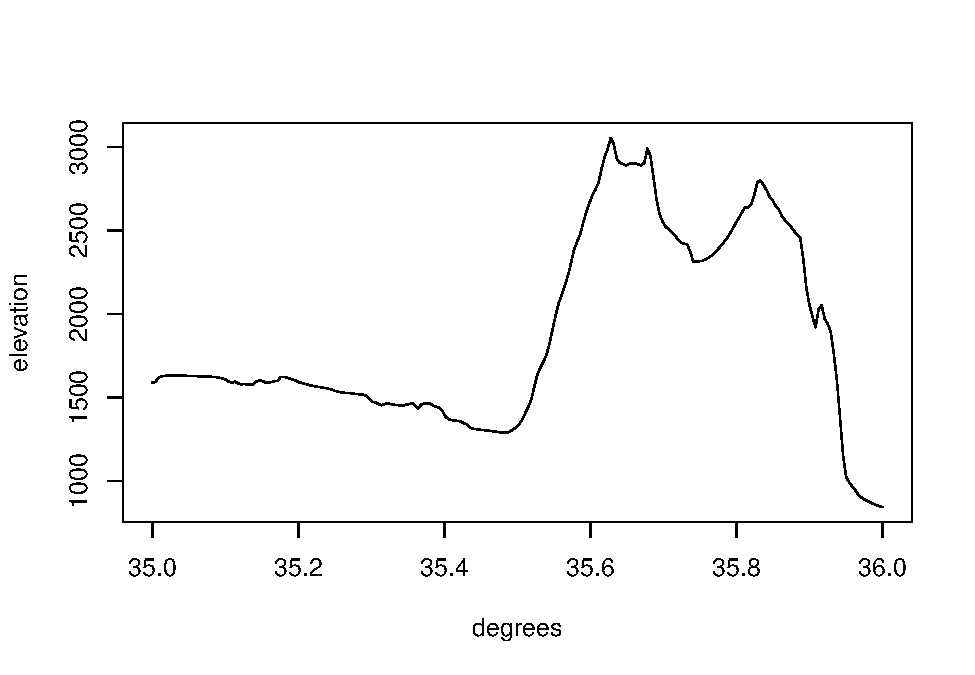
\includegraphics{_main_files/figure-latex/unnamed-chunk-16-1.pdf}

Oops! Our points are all sitting under the map of Brazil! This is the first thing we want to keep in mind: the ggplot object plots layers in order. If we want the points on top, they get added last.

\begin{Shaded}
\begin{Highlighting}[]
\CommentTok{\#Plot in correct order}
\NormalTok{primatePlot}\OtherTok{\textless{}{-}}\FunctionTok{ggplot}\NormalTok{() }\SpecialCharTok{+} 
  \FunctionTok{geom\_sf}\NormalTok{(}\AttributeTok{data=}\NormalTok{ states) }\SpecialCharTok{+}
  \FunctionTok{geom\_sf}\NormalTok{(}\AttributeTok{data =}\NormalTok{ brazilPrimates) }
\FunctionTok{print}\NormalTok{(primatePlot)}
\end{Highlighting}
\end{Shaded}

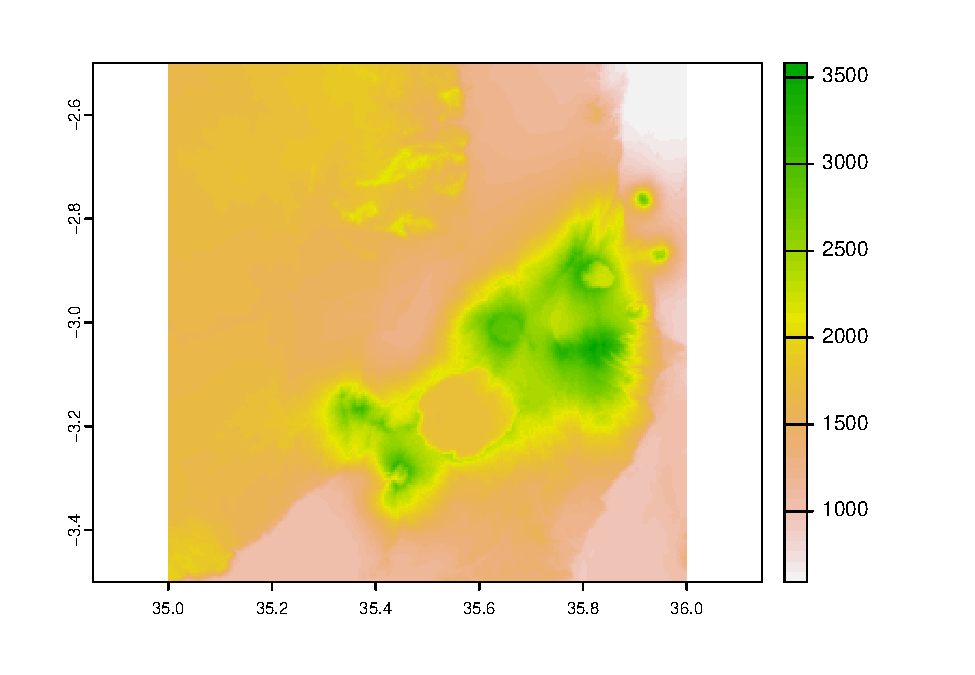
\includegraphics{_main_files/figure-latex/unnamed-chunk-17-1.pdf}

That's better. Now, let's give the states a different color.

\begin{Shaded}
\begin{Highlighting}[]
\CommentTok{\#Plot with title and axis labels}
\NormalTok{primatePlot}\OtherTok{\textless{}{-}}\FunctionTok{ggplot}\NormalTok{() }\SpecialCharTok{+} 
  \FunctionTok{geom\_sf}\NormalTok{(}\AttributeTok{data=}\NormalTok{ states, }\AttributeTok{fill=}\StringTok{"light green"}\NormalTok{) }\SpecialCharTok{+}
  \FunctionTok{scale\_color\_brewer}\NormalTok{(}\AttributeTok{palette=}\StringTok{"Paired"}\NormalTok{) }\SpecialCharTok{+}
  \FunctionTok{geom\_sf}\NormalTok{(}\AttributeTok{data =}\NormalTok{ brazilPrimates)}
\FunctionTok{print}\NormalTok{(primatePlot)}
\end{Highlighting}
\end{Shaded}

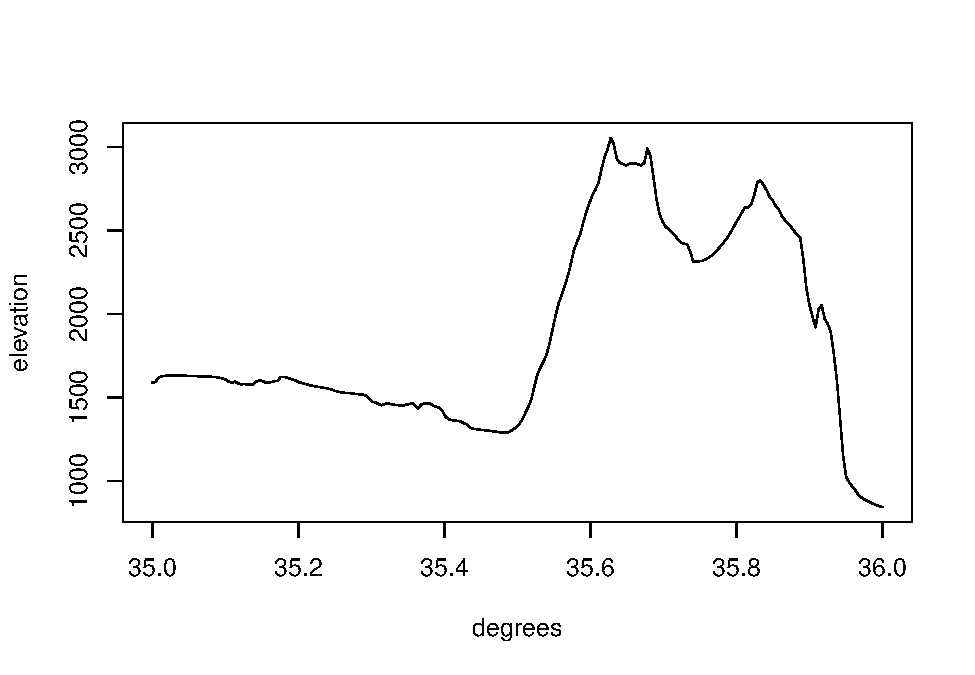
\includegraphics{_main_files/figure-latex/unnamed-chunk-18-1.pdf}

OK, now let's change the look of the primate data. Maybe we want to show the diversity of species in the dataset. Let's look at the data and find a good attribute for that:

\begin{Shaded}
\begin{Highlighting}[]
\FunctionTok{head}\NormalTok{(brazilPrimates)}
\end{Highlighting}
\end{Shaded}

\begin{verbatim}
## Simple feature collection with 6 features and 48 fields
## Geometry type: POINT
## Dimension:     XY
## Bounding box:  xmin: -48.10679 ymin: -22.98356 xmax: -40.06505 ymax: -15.56004
## Geodetic CRS:  WGS 84
##        gbifID                           datasetKey
## 22 3760406607 50c9509d-22c7-4a22-a47d-8c48425ef4a7
## 24 3760402428 50c9509d-22c7-4a22-a47d-8c48425ef4a7
## 30 3760386387 50c9509d-22c7-4a22-a47d-8c48425ef4a7
## 38 3760360787 50c9509d-22c7-4a22-a47d-8c48425ef4a7
## 40 3760350394 50c9509d-22c7-4a22-a47d-8c48425ef4a7
## 43 3760344838 50c9509d-22c7-4a22-a47d-8c48425ef4a7
##                                          occurrenceID  kingdom   phylum
## 22 https://www.inaturalist.org/observations/112156242 Animalia Chordata
## 24 https://www.inaturalist.org/observations/110912409 Animalia Chordata
## 30 https://www.inaturalist.org/observations/111860218 Animalia Chordata
## 38 https://www.inaturalist.org/observations/111202030 Animalia Chordata
## 40 https://www.inaturalist.org/observations/111853748 Animalia Chordata
## 43 https://www.inaturalist.org/observations/112298162 Animalia Chordata
##       class    order         family      genus                species
## 22 Mammalia Primates Callitrichidae Callithrix   Callithrix geoffroyi
## 24 Mammalia Primates Callitrichidae Callithrix Callithrix penicillata
## 30 Mammalia Primates    Pitheciidae Callicebus  Callicebus personatus
## 38 Mammalia Primates        Cebidae    Sapajus       Sapajus nigritus
## 40 Mammalia Primates Callitrichidae Callithrix   Callithrix geoffroyi
## 43 Mammalia Primates Callitrichidae Callithrix Callithrix penicillata
##    infraspecificEpithet taxonRank
## 22                        SPECIES
## 24                        SPECIES
## 30                        SPECIES
## 38                        SPECIES
## 40                        SPECIES
## 43                        SPECIES
##                                                scientificName
## 22                      Callithrix geoffroyi (Humboldt, 1812)
## 24 Callithrix penicillata (\xc9.Geoffroy Saint-Hilaire, 1812)
## 30  Callicebus personatus (\xc9.Geoffroy Saint-Hilaire, 1812)
## 38                          Sapajus nigritus (Goldfuss, 1809)
## 40                      Callithrix geoffroyi (Humboldt, 1812)
## 43 Callithrix penicillata (\xc9.Geoffroy Saint-Hilaire, 1812)
##    verbatimScientificName verbatimScientificNameAuthorship countryCode locality
## 22   Callithrix geoffroyi                                           BR         
## 24 Callithrix penicillata                                           BR         
## 30  Callicebus personatus                                           BR         
## 38       Sapajus nigritus                                           BR         
## 40   Callithrix geoffroyi                                           BR         
## 43 Callithrix penicillata                                           BR         
##        stateProvince occurrenceStatus individualCount
## 22 Esp\xedrito Santo          PRESENT              NA
## 24  Distrito Federal          PRESENT              NA
## 30 Esp\xedrito Santo          PRESENT              NA
## 38    Rio de Janeiro          PRESENT              NA
## 40 Esp\xedrito Santo          PRESENT              NA
## 43  Distrito Federal          PRESENT              NA
##                        publishingOrgKey coordinateUncertaintyInMeters
## 22 28eb1a3f-1c15-4a95-931a-4af90ecb574d                           970
## 24 28eb1a3f-1c15-4a95-931a-4af90ecb574d                           967
## 30 28eb1a3f-1c15-4a95-931a-4af90ecb574d                         30562
## 38 28eb1a3f-1c15-4a95-931a-4af90ecb574d                         30237
## 40 28eb1a3f-1c15-4a95-931a-4af90ecb574d                           464
## 43 28eb1a3f-1c15-4a95-931a-4af90ecb574d                             4
##    coordinatePrecision elevation elevationAccuracy depth depthAccuracy
## 22                  NA        NA                NA    NA            NA
## 24                  NA        NA                NA    NA            NA
## 30                  NA        NA                NA    NA            NA
## 38                  NA        NA                NA    NA            NA
## 40                  NA        NA                NA    NA            NA
## 43                  NA        NA                NA    NA            NA
##          eventDate day month year taxonKey speciesKey     basisOfRecord
## 22  6/5/2016 13:47   5     6 2016  5219539    5219539 HUMAN_OBSERVATION
## 24  4/9/2022 11:19   9     4 2022  5219541    5219541 HUMAN_OBSERVATION
## 30 2/16/2015 13:49  16     2 2015  2436398    2436398 HUMAN_OBSERVATION
## 38   4/7/2019 0:00   7     4 2019  7519053    7519053 HUMAN_OBSERVATION
## 40 12/1/2013 12:40   1    12 2013  5219539    5219539 HUMAN_OBSERVATION
## 43  4/21/2022 9:33  21     4 2022  5219541    5219541 HUMAN_OBSERVATION
##    institutionCode collectionCode catalogNumber recordNumber       identifiedBy
## 22     iNaturalist   Observations     112156242           NA      Gabriel Bonfa
## 24     iNaturalist   Observations     110912409           NA Enrico A. R. Tosto
## 30     iNaturalist   Observations     111860218           NA      Gabriel Bonfa
## 38     iNaturalist   Observations     111202030           NA     Michal Sloviak
## 40     iNaturalist   Observations     111853748           NA      Gabriel Bonfa
## 43     iNaturalist   Observations     112298162           NA    Maria Clara Gil
##     dateIdentified      license      rightsHolder        recordedBy typeStatus
## 22 4/20/2022 15:08 CC_BY_NC_4_0     Gabriel Bonfa     Gabriel Bonfa           
## 24  4/10/2022 1:04 CC_BY_NC_4_0  abelardomendesjr  abelardomendesjr           
## 30  4/18/2022 0:02 CC_BY_NC_4_0     Gabriel Bonfa     Gabriel Bonfa           
## 38 4/12/2022 15:13 CC_BY_NC_4_0 Wagner Fiorentino Wagner Fiorentino           
## 40 4/17/2022 23:08 CC_BY_NC_4_0     Gabriel Bonfa     Gabriel Bonfa           
## 43 4/21/2022 18:50 CC_BY_NC_4_0   Maria Clara Gil   Maria Clara Gil           
##    establishmentMeans lastInterpreted  mediaType              issue
## 22                     5/2/2022 16:23 StillImage COORDINATE_ROUNDED
## 24                     5/2/2022 15:55 StillImage COORDINATE_ROUNDED
## 30                     5/2/2022 14:50 StillImage COORDINATE_ROUNDED
## 38                     5/2/2022 16:04 StillImage COORDINATE_ROUNDED
## 40                     5/2/2022 16:18 StillImage COORDINATE_ROUNDED
## 43                     5/2/2022 16:26 StillImage COORDINATE_ROUNDED
##                       geometry
## 22 POINT (-40.06505 -19.15138)
## 24 POINT (-47.86165 -15.73703)
## 30  POINT (-40.32546 -19.4921)
## 38 POINT (-43.20546 -22.98355)
## 40  POINT (-40.2999 -19.40386)
## 43 POINT (-48.10679 -15.56004)
\end{verbatim}

OK, let's go with \texttt{genus}. To access this for plotting, we need to tell ggplot that this will be used as an aesthetic, so we call \texttt{aes}. Everything we ask for inside \texttt{aes} will be evaluated for each point, while everything outside that call gets applied the same way to all points.

\begin{Shaded}
\begin{Highlighting}[]
\CommentTok{\#Plot with title and axis labels}
\NormalTok{primatePlot}\OtherTok{\textless{}{-}}\FunctionTok{ggplot}\NormalTok{() }\SpecialCharTok{+} 
  \FunctionTok{geom\_sf}\NormalTok{(}\AttributeTok{data=}\NormalTok{ states, }\AttributeTok{fill=}\StringTok{"light green"}\NormalTok{) }\SpecialCharTok{+}
  \FunctionTok{scale\_color\_brewer}\NormalTok{(}\AttributeTok{palette=}\StringTok{"Paired"}\NormalTok{) }\SpecialCharTok{+}
  \FunctionTok{geom\_sf}\NormalTok{(}\AttributeTok{data =}\NormalTok{ brazilPrimates,}\FunctionTok{aes}\NormalTok{(}\AttributeTok{color=}\NormalTok{genus))}
\FunctionTok{print}\NormalTok{(primatePlot)}
\end{Highlighting}
\end{Shaded}

\begin{verbatim}
## Warning in RColorBrewer::brewer.pal(n, pal): n too large, allowed maximum for palette Paired is 12
## Returning the palette you asked for with that many colors
\end{verbatim}

\begin{verbatim}
## Warning: Removed 2077 rows containing missing values (geom_sf).
\end{verbatim}

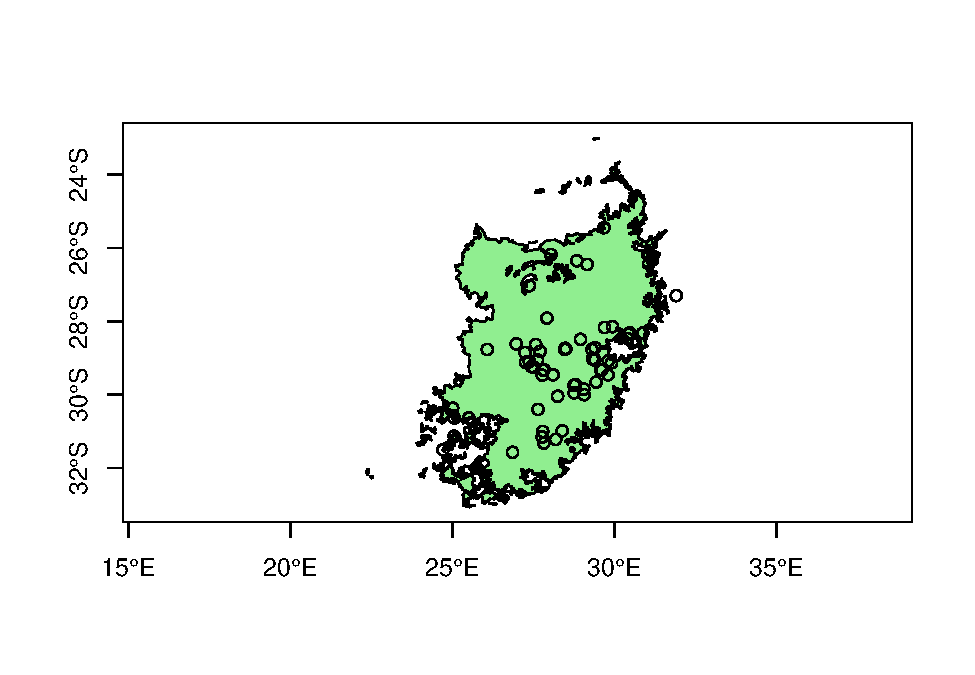
\includegraphics{_main_files/figure-latex/unnamed-chunk-20-1.pdf}

Ack! The giant legend strikes again! There's a couple more problems here. First, there's a bunch of points that don't have a value for genus. And second we ran out of colors! We could find other ways to get more colors, but all of these problems could potentially be solved by plotting by \texttt{family} instead.

\begin{Shaded}
\begin{Highlighting}[]
\CommentTok{\#Plot with title and axis labels}
\NormalTok{primatePlot}\OtherTok{\textless{}{-}}\FunctionTok{ggplot}\NormalTok{() }\SpecialCharTok{+} 
  \FunctionTok{geom\_sf}\NormalTok{(}\AttributeTok{data=}\NormalTok{ states, }\AttributeTok{fill=}\StringTok{"light green"}\NormalTok{) }\SpecialCharTok{+}
  \FunctionTok{scale\_color\_brewer}\NormalTok{(}\AttributeTok{palette=}\StringTok{"Paired"}\NormalTok{) }\SpecialCharTok{+}
  \FunctionTok{geom\_sf}\NormalTok{(}\AttributeTok{data =}\NormalTok{ brazilPrimates,}\FunctionTok{aes}\NormalTok{(}\AttributeTok{color=}\NormalTok{family))}
\FunctionTok{print}\NormalTok{(primatePlot)}
\end{Highlighting}
\end{Shaded}

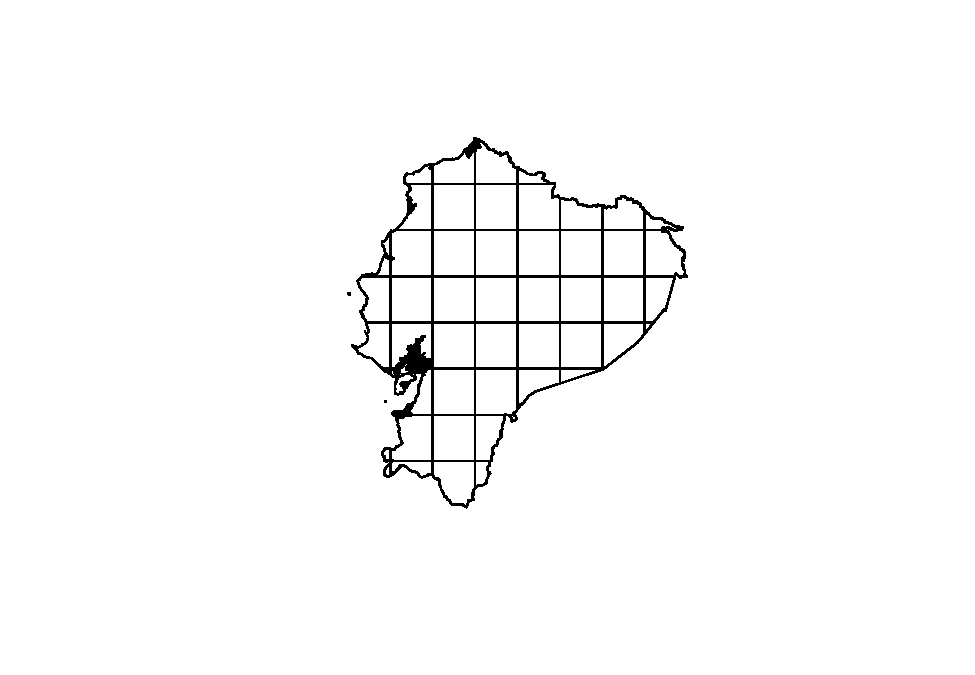
\includegraphics{_main_files/figure-latex/unnamed-chunk-21-1.pdf}

Much better. There's a couple of points here where family was recorded as ``\,``, so those have no label. We can eliminate those quickly with \texttt{subset}:

\begin{Shaded}
\begin{Highlighting}[]
\NormalTok{brazilPrimates}\OtherTok{\textless{}{-}}\FunctionTok{subset}\NormalTok{(brazilPrimates,family }\SpecialCharTok{!=} \StringTok{""}\NormalTok{)}
\end{Highlighting}
\end{Shaded}

Also, someone apparently took the time to send in some observations of Hominidae! We'll leave that one in there. Ecologists are a fun bunch.

Let's wrap this section up by adding some axis labels and a title.

\begin{Shaded}
\begin{Highlighting}[]
\CommentTok{\#Plot with title and axis labels}
\NormalTok{primatePlot}\OtherTok{\textless{}{-}}\FunctionTok{ggplot}\NormalTok{() }\SpecialCharTok{+} 
  \FunctionTok{geom\_sf}\NormalTok{(}\AttributeTok{data=}\NormalTok{ states, }\AttributeTok{fill=}\StringTok{"light green"}\NormalTok{) }\SpecialCharTok{+}
  \FunctionTok{scale\_color\_brewer}\NormalTok{(}\AttributeTok{palette=}\StringTok{"Paired"}\NormalTok{) }\SpecialCharTok{+}
  \FunctionTok{geom\_sf}\NormalTok{(}\AttributeTok{data =}\NormalTok{ brazilPrimates,}\FunctionTok{aes}\NormalTok{(}\AttributeTok{color=}\NormalTok{family)) }\SpecialCharTok{+}
  \FunctionTok{labs}\NormalTok{(}\AttributeTok{x=}\StringTok{"Longitude"}\NormalTok{,}\AttributeTok{y=}\StringTok{"Latitude"}\NormalTok{,}\AttributeTok{title=}\StringTok{"Primate Observations in Brazil"}\NormalTok{)}
\FunctionTok{print}\NormalTok{(primatePlot)}
\end{Highlighting}
\end{Shaded}

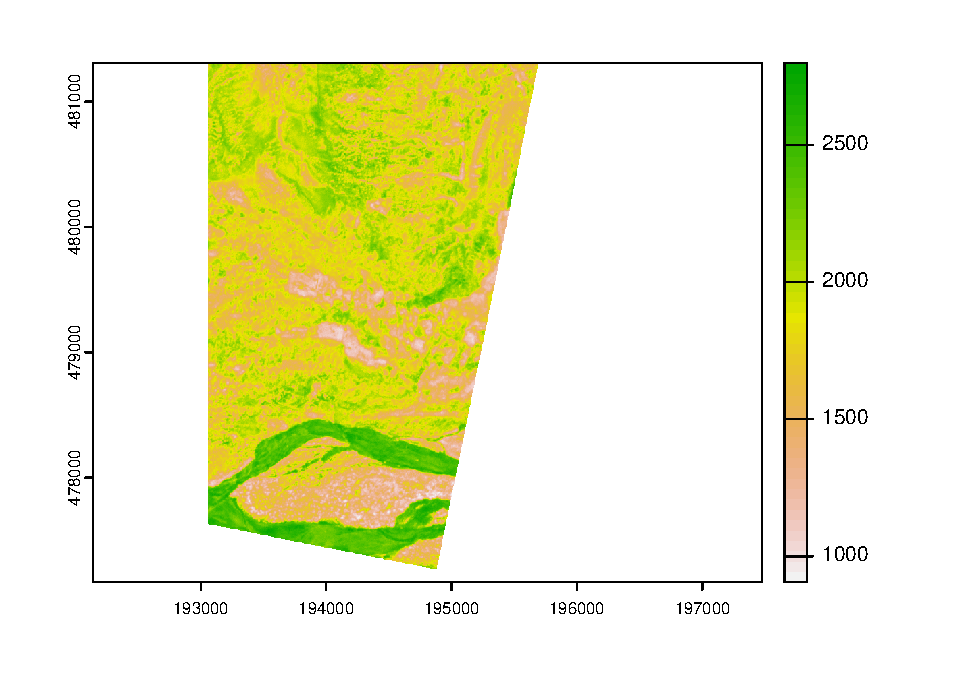
\includegraphics{_main_files/figure-latex/unnamed-chunk-23-1.pdf}

\hypertarget{adding-map-elements}{%
\chapter{Adding map elements}\label{adding-map-elements}}

In addition to the plot itself, we want to make sure we're able to add other necessary plot elements. To get access to these, we'll use the \texttt{ggspatial} package.

Let's start with a north arrow:

\begin{Shaded}
\begin{Highlighting}[]
\CommentTok{\#Plot with title and axis labels}
\NormalTok{primatePlot}\OtherTok{\textless{}{-}}\FunctionTok{ggplot}\NormalTok{() }\SpecialCharTok{+} 
  \FunctionTok{geom\_sf}\NormalTok{(}\AttributeTok{data=}\NormalTok{ states, }\AttributeTok{fill=}\StringTok{"light green"}\NormalTok{) }\SpecialCharTok{+}
  \FunctionTok{scale\_color\_brewer}\NormalTok{(}\AttributeTok{palette=}\StringTok{"Paired"}\NormalTok{) }\SpecialCharTok{+}
  \FunctionTok{geom\_sf}\NormalTok{(}\AttributeTok{data =}\NormalTok{ brazilPrimates,}\FunctionTok{aes}\NormalTok{(}\AttributeTok{color=}\NormalTok{family)) }\SpecialCharTok{+}
  \FunctionTok{labs}\NormalTok{(}\AttributeTok{x=}\StringTok{"Longitude"}\NormalTok{,}\AttributeTok{y=}\StringTok{"Latitude"}\NormalTok{,}\AttributeTok{title=}\StringTok{"Primate Observations in Brazil"}\NormalTok{)  }\SpecialCharTok{+}
   \FunctionTok{annotation\_north\_arrow}\NormalTok{(}\AttributeTok{location =} \StringTok{"bl"}\NormalTok{,  }\AttributeTok{height =} \FunctionTok{unit}\NormalTok{(}\DecValTok{1}\NormalTok{, }\StringTok{"cm"}\NormalTok{), }\AttributeTok{width =} \FunctionTok{unit}\NormalTok{(}\DecValTok{1}\NormalTok{, }\StringTok{"cm"}\NormalTok{),}\AttributeTok{pad\_x =} \FunctionTok{unit}\NormalTok{(}\FloatTok{0.1}\NormalTok{, }\StringTok{"cm"}\NormalTok{), }\AttributeTok{pad\_y =} \FunctionTok{unit}\NormalTok{(}\FloatTok{0.1}\NormalTok{, }\StringTok{"cm"}\NormalTok{),}\AttributeTok{style =}\NormalTok{ north\_arrow\_fancy\_orienteering)}


\FunctionTok{print}\NormalTok{(primatePlot)}
\end{Highlighting}
\end{Shaded}

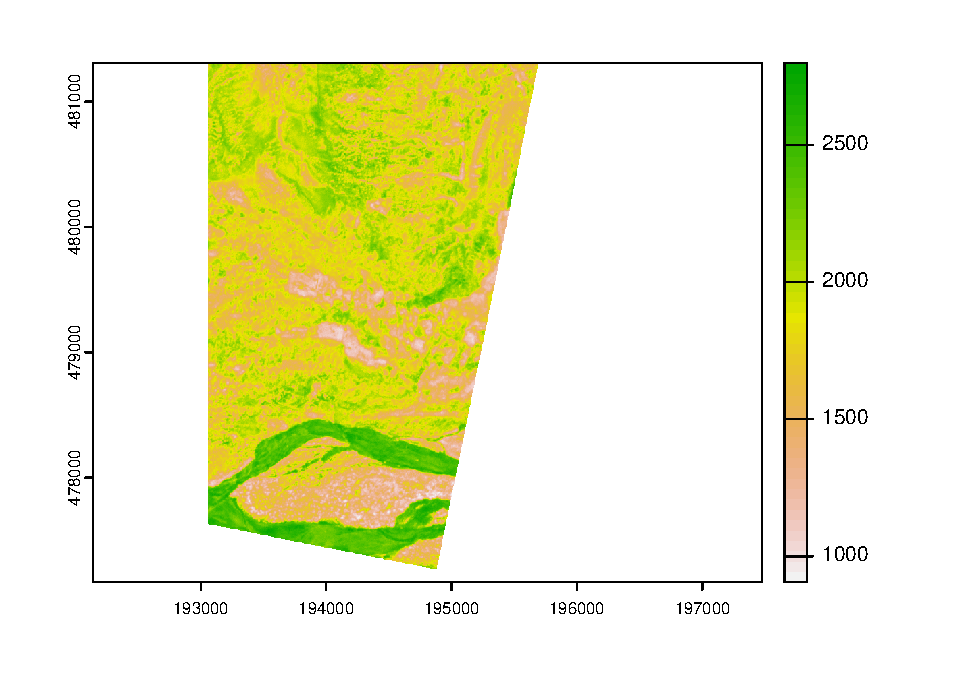
\includegraphics{_main_files/figure-latex/unnamed-chunk-24-1.pdf}

Looks pretty good. There are a number of parameters here that control how big it is, where it is on the page, and what kind of arrow it is. Let's move it from the bottom left (\texttt{\textquotesingle{}bl\textquotesingle{}}) to the top right (\texttt{\textquotesingle{}tr\textquotesingle{}}) with the \texttt{location} parameter:

\begin{Shaded}
\begin{Highlighting}[]
\CommentTok{\#Plot with title and axis labels}
\NormalTok{primatePlot}\OtherTok{\textless{}{-}}\FunctionTok{ggplot}\NormalTok{() }\SpecialCharTok{+} 
  \FunctionTok{geom\_sf}\NormalTok{(}\AttributeTok{data=}\NormalTok{ states, }\AttributeTok{fill=}\StringTok{"light green"}\NormalTok{) }\SpecialCharTok{+}
  \FunctionTok{scale\_color\_brewer}\NormalTok{(}\AttributeTok{palette=}\StringTok{"Paired"}\NormalTok{) }\SpecialCharTok{+}
  \FunctionTok{geom\_sf}\NormalTok{(}\AttributeTok{data =}\NormalTok{ brazilPrimates,}\FunctionTok{aes}\NormalTok{(}\AttributeTok{color=}\NormalTok{family)) }\SpecialCharTok{+}
  \FunctionTok{labs}\NormalTok{(}\AttributeTok{x=}\StringTok{"Longitude"}\NormalTok{,}\AttributeTok{y=}\StringTok{"Latitude"}\NormalTok{,}\AttributeTok{title=}\StringTok{"Primate Observations in Brazil"}\NormalTok{)  }\SpecialCharTok{+}
   \FunctionTok{annotation\_north\_arrow}\NormalTok{(}\AttributeTok{location =} \StringTok{"tr"}\NormalTok{,  }\AttributeTok{height =} \FunctionTok{unit}\NormalTok{(}\DecValTok{1}\NormalTok{, }\StringTok{"cm"}\NormalTok{), }\AttributeTok{width =} \FunctionTok{unit}\NormalTok{(}\DecValTok{1}\NormalTok{, }\StringTok{"cm"}\NormalTok{),}\AttributeTok{pad\_x =} \FunctionTok{unit}\NormalTok{(}\FloatTok{0.1}\NormalTok{, }\StringTok{"cm"}\NormalTok{), }\AttributeTok{pad\_y =} \FunctionTok{unit}\NormalTok{(}\FloatTok{0.1}\NormalTok{, }\StringTok{"cm"}\NormalTok{),}\AttributeTok{style =}\NormalTok{ north\_arrow\_fancy\_orienteering)}


\FunctionTok{print}\NormalTok{(primatePlot)}
\end{Highlighting}
\end{Shaded}

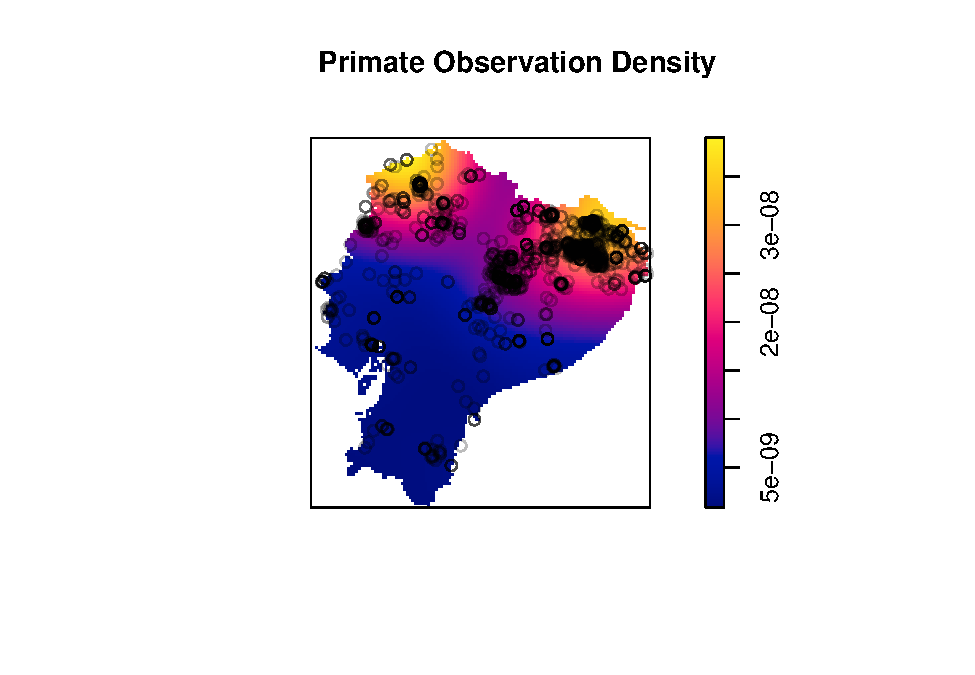
\includegraphics{_main_files/figure-latex/unnamed-chunk-25-1.pdf}

We can probably do with a less fancy north arrow, frankly. You can find the different arrows (and the parameters that control them) by running \texttt{?north\_arrow\_orienteering} Lets go with \texttt{north\_arrow\_minimal} here.

\begin{Shaded}
\begin{Highlighting}[]
\CommentTok{\#Plot with title and axis labels}
\NormalTok{primatePlot}\OtherTok{\textless{}{-}}\FunctionTok{ggplot}\NormalTok{() }\SpecialCharTok{+} 
  \FunctionTok{geom\_sf}\NormalTok{(}\AttributeTok{data=}\NormalTok{ states, }\AttributeTok{fill=}\StringTok{"light green"}\NormalTok{) }\SpecialCharTok{+}
  \FunctionTok{scale\_color\_brewer}\NormalTok{(}\AttributeTok{palette=}\StringTok{"Paired"}\NormalTok{) }\SpecialCharTok{+}
  \FunctionTok{geom\_sf}\NormalTok{(}\AttributeTok{data =}\NormalTok{ brazilPrimates,}\FunctionTok{aes}\NormalTok{(}\AttributeTok{color=}\NormalTok{family)) }\SpecialCharTok{+}
  \FunctionTok{labs}\NormalTok{(}\AttributeTok{x=}\StringTok{"Longitude"}\NormalTok{,}\AttributeTok{y=}\StringTok{"Latitude"}\NormalTok{,}\AttributeTok{title=}\StringTok{"Primate Observations in Brazil"}\NormalTok{)  }\SpecialCharTok{+}
   \FunctionTok{annotation\_north\_arrow}\NormalTok{(}\AttributeTok{location =} \StringTok{"tr"}\NormalTok{,  }\AttributeTok{height =} \FunctionTok{unit}\NormalTok{(}\DecValTok{1}\NormalTok{, }\StringTok{"cm"}\NormalTok{), }\AttributeTok{width =} \FunctionTok{unit}\NormalTok{(}\DecValTok{1}\NormalTok{, }\StringTok{"cm"}\NormalTok{),}\AttributeTok{pad\_x =} \FunctionTok{unit}\NormalTok{(}\FloatTok{0.1}\NormalTok{, }\StringTok{"cm"}\NormalTok{), }\AttributeTok{pad\_y =} \FunctionTok{unit}\NormalTok{(}\FloatTok{0.1}\NormalTok{, }\StringTok{"cm"}\NormalTok{),}\AttributeTok{style =}\NormalTok{ north\_arrow\_minimal)}


\FunctionTok{print}\NormalTok{(primatePlot)}
\end{Highlighting}
\end{Shaded}

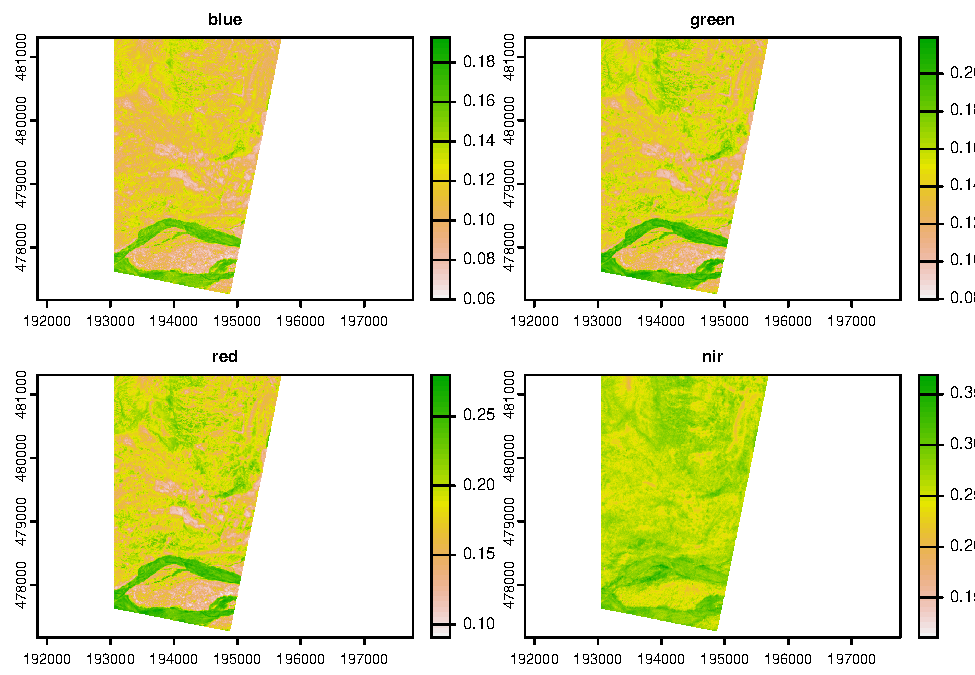
\includegraphics{_main_files/figure-latex/unnamed-chunk-26-1.pdf}

Classy. Finally, our map needs a scale bar. We add that with \texttt{annotation\_scale}:

\begin{Shaded}
\begin{Highlighting}[]
\CommentTok{\#Plot with title and axis labels}
\NormalTok{primatePlot}\OtherTok{\textless{}{-}}\FunctionTok{ggplot}\NormalTok{() }\SpecialCharTok{+} 
  \FunctionTok{geom\_sf}\NormalTok{(}\AttributeTok{data=}\NormalTok{ states, }\AttributeTok{fill=}\StringTok{"light green"}\NormalTok{) }\SpecialCharTok{+}
  \FunctionTok{scale\_color\_brewer}\NormalTok{(}\AttributeTok{palette=}\StringTok{"Paired"}\NormalTok{) }\SpecialCharTok{+}
  \FunctionTok{geom\_sf}\NormalTok{(}\AttributeTok{data =}\NormalTok{ brazilPrimates,}\FunctionTok{aes}\NormalTok{(}\AttributeTok{color=}\NormalTok{family)) }\SpecialCharTok{+}
  \FunctionTok{labs}\NormalTok{(}\AttributeTok{x=}\StringTok{"Longitude"}\NormalTok{,}\AttributeTok{y=}\StringTok{"Latitude"}\NormalTok{,}\AttributeTok{title=}\StringTok{"Primate Observations in Brazil"}\NormalTok{)  }\SpecialCharTok{+}
    \FunctionTok{annotation\_north\_arrow}\NormalTok{(}\AttributeTok{location =} \StringTok{"tr"}\NormalTok{,  }\AttributeTok{height =} \FunctionTok{unit}\NormalTok{(}\DecValTok{1}\NormalTok{, }\StringTok{"cm"}\NormalTok{), }\AttributeTok{width =} \FunctionTok{unit}\NormalTok{(}\DecValTok{1}\NormalTok{, }\StringTok{"cm"}\NormalTok{),}\AttributeTok{pad\_x =} \FunctionTok{unit}\NormalTok{(}\FloatTok{0.1}\NormalTok{, }\StringTok{"cm"}\NormalTok{), }\AttributeTok{pad\_y =} \FunctionTok{unit}\NormalTok{(}\FloatTok{0.1}\NormalTok{, }\StringTok{"cm"}\NormalTok{),}\AttributeTok{style =}\NormalTok{ north\_arrow\_minimal) }\SpecialCharTok{+}
\FunctionTok{annotation\_scale}\NormalTok{(}\AttributeTok{location =} \StringTok{"br"}\NormalTok{, }\AttributeTok{height =} \FunctionTok{unit}\NormalTok{(}\FloatTok{0.2}\NormalTok{, }\StringTok{"cm"}\NormalTok{)) }


\FunctionTok{print}\NormalTok{(primatePlot)}
\end{Highlighting}
\end{Shaded}

\begin{verbatim}
## Scale on map varies by more than 10%, scale bar may be inaccurate
\end{verbatim}

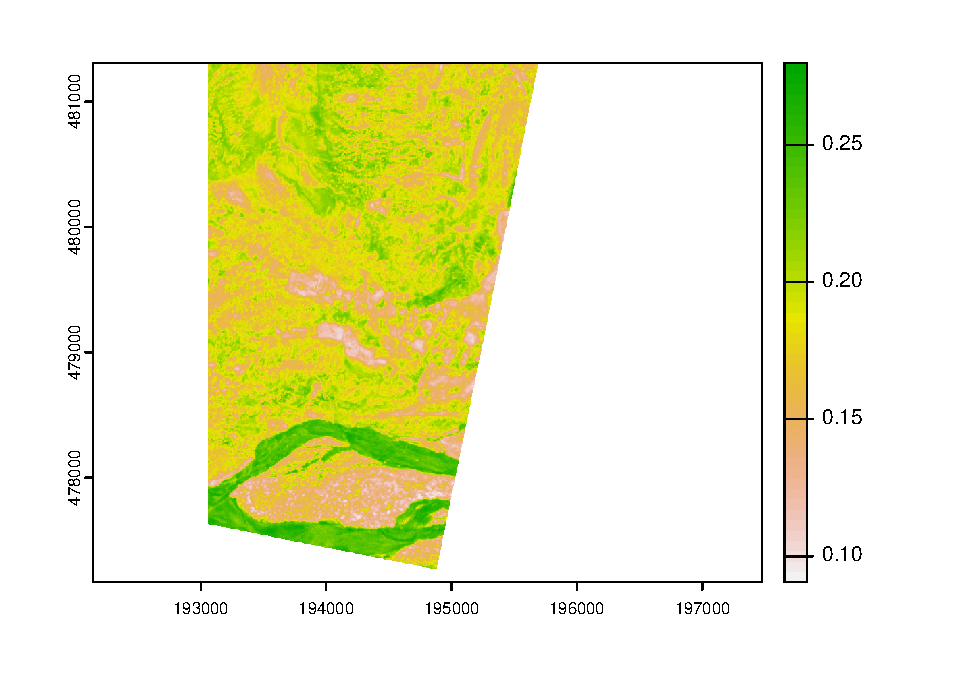
\includegraphics{_main_files/figure-latex/unnamed-chunk-27-1.pdf}

Notice that error? That's because we're plotting this using a Geographic (elliptical) coordinate system, but it's being plotted on a 2D plane. That means that the distance relationships vary somewhat across the map. The \texttt{ggspatial} package does it's best job to find a reasonable middle point for the scale, but it lets us know that we need to be careful.

\hypertarget{bringing-it-all-together}{%
\chapter{Bringing it all together}\label{bringing-it-all-together}}

Working with spatial data often involves finding a sequence of steps to create a desired endproduct. For this exercise, make a map of primate observations in Ecuador, with observations plotted by year. Use the data available in the working directory. Play around with a few different options for appearances, and don't forget to include a north arrow and scale bar!

  \bibliography{book.bib,packages.bib}

\end{document}
